\chapter{User Study}
In order to develop a device which can recognise the exercises, a lot of software development and research needed to be performed. However, the group felt an initial important step was to gather training data on which to base the development of an algorithm.

The data which is involved are the readings from sensors which are attached to the body of a person when they are performing the exercises. As it is the intention for the system to be used by many different people who travel in planes, it was decided to gather the training data using a user study. This is because each individual has slight variations in the way they perform exercises so in order to improve the robustness of the system we collected movement data from 20 different people. This movement data could then be combined as the training data to form a model capable of correctly classifying exercises for most people.

\namedsection{Study Preparation}{Finch}
Before performing studies involving participants who are not actually members of the project it is required to gain ethical approval. This is a requirement put in place from the University of Southampton and also covers the legal requirement of data protection when dealing with participant's personal data. Faculty ethics committees review applications for ethical approval and once they are approved insurance and legal cover is provided. Therefore, it is highly important to follow the approval process as it helps to make sure there is enough detail and planning in the study to help keep participants safe.

To get advice with the application process, contact was made with the University of Southampton Safety and Occupational Health department (SOH) \cite{sotonsoh}. In a meeting between the groups user study lead and members of SOH it was decided that the study should take place in a private room where there would not be any interruptions and assistance was provided with booking a lab room in the Psychology department for this purpose. Further assistance was also given for finding the contact details of first aiders.

\namedsection{Ethical Approval Process}{Finch}
Throughout the application process, heavy reference was made to the instructions and guideline documents provided by the Ethics and Research Governance Online website \cite{ergo}. One of the key things that are used to classify studies are study characteristics which are a list of areas where potential risks could be introduced ranging from low to high likelihood. As our study involved wearable technology, this counted as being intrusive which in turn meant there was a risk of harm and these are two medium risk study characteristics.

This meant that the user study had to provide consent forms so that participants could provide their consent for taking part in writing. However, this also meant that personal data was collected in the study which caused another study characteristic to be matched.

Overall, this required several documents to be submitted as part of the ethics application. These included the consent form as already mentioned and participant information which clearly stated to the participants what will be required of them in the study. On top of this, a data protection act plan which outlined how participant's personal data will be kept safe was also submitted along with a risk management plan which had to identify possible ways a participant might get injured and how these risks would be reduced. A debrief plan which stated how participants could be told of the results of the study was also included as were contact information and technical details documents to provide even further details about the study.

In this project, there were two areas where user studies could have been required. One was to collect movement data to train the algorithm by generating a model as already mentioned. The other area was to perform a user study to test the final system and measure its accuracy. As applying for ethics approval is a very time consuming process, it was decided to incorporate both areas into a single study. This was possible because both areas involve the participants performing exactly the same actions, it was only what was being recorded that changed. This was made clear throughout the ethics application which eventually led to it being approved.

\namedsection{First User Study}{Finch}
The first area of the user study was performed to collect movement data to train the algorithm. Specifically, accelerometer and gyroscope sensor data was required to be collected so that the effectiveness of the two at training the algorithm and accurately classifying exercises could be compared.

Appendix \ref{app:participant} shows the plan for the data gathering sessions along with instructions on what should be done for each participant.

\subsection{Recording Device}
At this stage in the project, the prototype device was not yet ready to be used to record the movement data so a mobile phone with inbuilt accelerometer and gyroscope sensor was used instead. The Physics Toolbox Suite Version 1.4.4 App \cite{vieyra2016} was used to record data directly from the phones sensors by allowing us to choose which sensors to use.

Initially, the plan was to record both accelerometer and gyroscope sensor data at the same time. This would save time as the participant would not have to repeat the exercise for each type of sensor. However, after the first two participants, it was quickly realised that the recorded data was of a poor quality as shown in figure \ref{fig:bad-data}.

\begin{figure}
	\centering
	\includegraphics[width=70mm]{figures/data-jump.pdf}
	\caption{Poor data collection showing unstable sampling frequency\label{fig:bad-data}}
\end{figure}

This is a result of unstable sampling from the phone as it was not powerful enough to sample data from both sensors at the same time at the highest frequency. Unfortunately, these sets of data were unusable to train the algorithm so the problem had to be rectified immediately before the next participant. The solution was to record from each sensor separately. The downside of this is that it doubled the time it took to collect the data.

\subsection{Performing the Recording}
For each participant, the phone was strapped to various parts of their body using Velcro. These positions included the top of the right foot, and the outer side of their upper right arm. It was also made sure that these positions and the orientation of the phone were the same for each participant in order to make sure the data was consistent. This was vital as the data from each participant was combined to form the overall training data.

When the phone was attached to the foot, each participant was sitting and performed the foot rotation exercises where they stretched out their legs and slowly rotated their feet in both clockwise and anticlockwise directions about 10 times each. Also while sitting down, each participant performed the ballerina exercise where they placed their feet on the ground and raised their heels, followed by raising their toes and rolling back their heels to the ground. This was also repeated about 10 times. Walking movement data was also collected while the phone was on the foot. It was important to collect this non-exercise movement data also; this was used as a cross reference when training the algorithm, to ensure the rate of false positives is suitably low.

When the phone was attached to the arm, the participants were told to do the shoulder rolling exercise where the shoulders were rolled forwards approximately 10 times.

Each of these exercises was repeated twice. One time for the accelerometer data and one for the gyroscope data. At the end of each exercise, the results were emailed to a member of the group who made them available on a Git repository.

\namedsection{Second User Study}{Finch}
In the end, the second part of the user study was not carried out due to the fact there was not sufficient time after the Christmas break to test the system with another complete user study. From the first user study, we knew it would take a long time to arrange and carry out when there is such a large group of people involved. This is because it can take a few weeks to find enough people willing to participate and who are available at the appropriate time. Furthermore, the study itself can take several days to perform. 

While testing the accuracy of the system is a vital part of the project, there were alternative ways to carry out the testing rather than performing a whole user study. This is why it was decided it was more feasible to drop the second user study and instead use the members of the project to test the system. The results of this can be seen in section \ref{sec:alg-accuracy}

\namedsection{Classification of Results}{Finch}
Once the first user study had been completed, the data collected from it needed to be manually classified. This is because a machine learning algorithm needs to be explicitly told what each piece of individual data means in order for it to use that as training data to create a model. In theory, when it is presented with new data it has not seen before, it will classify it based on how similar training data was manually classified.

As will be discussed in section \ref{sec:trade-off-parameters}, three separate classification classes were decided upon. These were “not exercise” for any activity that is not part of an exercise and “peaks” and “troughs” for activities that were exercises. 

\begin{figure}
	\centering
	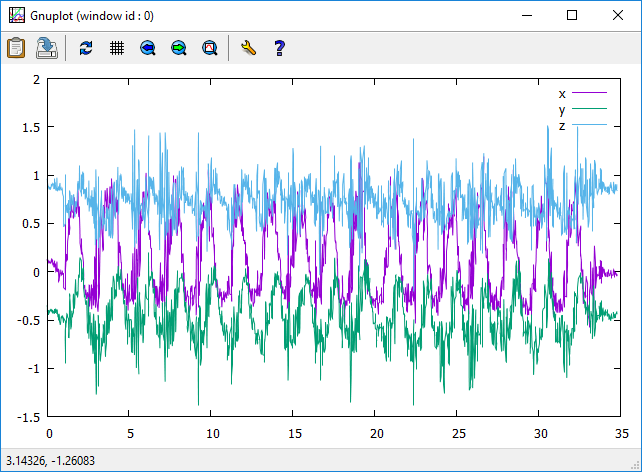
\includegraphics[width=1.0\textwidth]{figures/classification_data_plot.png}
	\caption{Gnuplot of accelerometer data for an anticlockwise revolver exercise\label{fig:gnuplot-rev}}
\end{figure}

Figure \ref{fig:gnuplot-rev} shows a plot of the accelerometer sensor data for one of the revolver exercises performed anticlockwise. The periodic motion of the exercise clearly translates to a series of peaks and troughs in the data.

These peaks and troughs are present in all of the dimensions (x, y, and z) but are certainly more distinct in some compared to others.  For example, for the accelerometer revolver data, the x axis showed the peaks and troughs best overall.

To perform the manual classification, each set of data was opened in Gnuplot, as shown in figure \ref{fig:gnuplot-rev}. Gnuplot is a tool which is capable of plotting data in any sort of format. The data received from the phone was in a simple CSV format so it was easy to instruct Gnuplot on how to plot this. As the mouse is moved across the plot, the precise coordinates of the mouse relative to the data in the plot is reported on screen. 

The manual classification involved first deciding which dimension to use (in this example the x dimension) and then moving the mouse pointer to every peak and trough in the data and recording the x-axis coordinates of each one.

This process was aided by the use of a simple Bash script which took the name of the file currently being classified, whether or not a peak or trough was being classified and then a list of x-axis coordinates of the location of those peaks and troughs. The script then output the results in a suitable format which could be read later on to be used to train the algorithm and generate the model.

Overall, there were about 20 sets of data that needed to be classified (a set of data from each participant). Each set included the revolver exercise (both clockwise and anticlockwise), the ballerina exercise and the shoulder rolling exercise. On top of this, each type of exercise is duplicated for both the accelerometer data and gyroscope data. This results in nearly 160 separate data plots to be manually classified.

As can be imagined, this was quite a time consuming process. Fortunately, for the vast majority of data plots, the peaks and troughs were very clear so it did not take very long to jot down their coordinates. Sometimes, the peaks and troughs were much harder to locate in the data which did increase the manual classification time.

Finally, the classification of the “not exercise” class did not need to be performed manually. This is because unlike the exercise classes, there was no need to distinguish different types of non-exercise. Instead, a script was used to mark periodic coordinates of the data as not exercise.
